\documentclass[11pt]{article}
\usepackage[a4paper,margin=1.8cm]{geometry}
\usepackage{amsmath, amssymb, amsthm}  % Essential math packages
\usepackage{graphicx}                   % For figures
\usepackage{hyperref}                   % Clickable links
\usepackage{parskip} % cleaner spacing
\usepackage{enumitem}
\usepackage{mdframed}
\usepackage{titlesec}
\newcommand{\sectionbreak}{\clearpage}

\usepackage{listings}
\usepackage{xcolor}



\lstset{
  language=Python,
  basicstyle=\ttfamily\small,
  keywordstyle=\color{blue},
  stringstyle=\color{red},
  commentstyle=\color{green!50!black},
  showstringspaces=false,
  breaklines=true
}

% Define a solution environment with a box
\newenvironment{solbox}
  {\begin{mdframed}[linewidth=1pt,linecolor=black,roundcorner=5pt]
   \noindent\textbf{Ans: }\enspace}
  {\end{mdframed}}


\title{Assigment 1 \\ MAT3110 - Introduction to numerical analysis}
\author{Oliver Ekeberg}
\date{\today}

\begin{document}
\maketitle


\tableofcontents

\section{Exercise 1}

Use the QR factorization of A and apply back substitution to R1 to
find x. You will need to write your own routine for back substitution
but you can use the matlab function
[Q,R] = qr(A);
to find Q and R.


\begin{solbox}

    \subsection{Back-substitution implementation}
    

    I used the built in function for Q and R calculations from numpy. I implemented the following function for back substitution:

    \begin{lstlisting}[language=Python]
        def back_subst(A: np.ndarray, b: np.ndarray):
            n = b.shape[0]
            if A.shape[0] != A.shape[1]:
                raise ValueError("Input must be square, douche...")
            x = np.zeros(n)
            x[n-1] = b[n-1] / A[n-1, n-1]

            for i in range(n-2, -1, -1):
                x[i] =  (b[i] - A[i, i+1:] @ x[i+1:]) / A[i,i]
            return x
    \end{lstlisting}
    \begin{itemize}
        \item The code takes input square a upper triangle matrix, and an arbitrary vector b that takes the same shape as the rows and columns of A
        \item Then I loop backwards from the lower diagonal and up. I have equations of the following form
        \[
            \sum_{ j=n }^{ n-j } \sum_{ i=j+1 }^{ j=n } a_{ji} x_j = b_j 
        \]
        And we can solve this by taking the dot product of th
        
    
    \end{itemize}
    


    \subsection{QR plot for dataset 1 m=3}
    
    This produced the following plot for data set 1:

    \begin{center}
    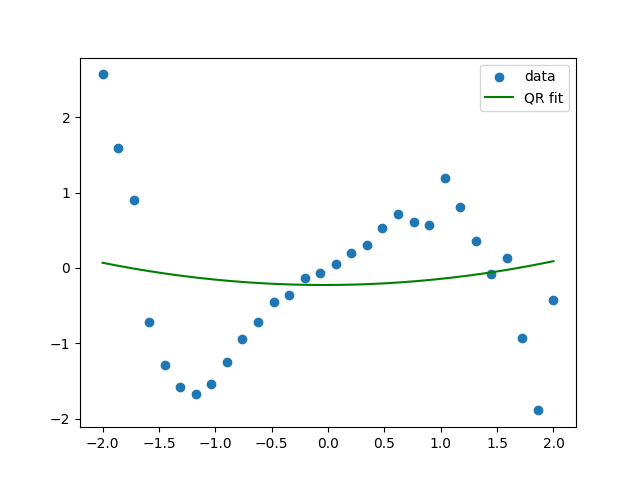
\includegraphics[width=0.75\linewidth]{../Figures/M3QR_plot_dataset1.png}
    \end{center}

    \subsection{QR plot for dataset 2 m=3}
    
    And the following plot for dataset 2:
    \begin{center}
    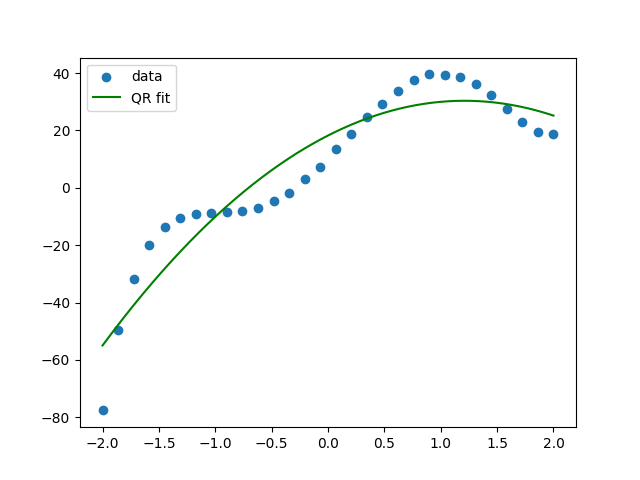
\includegraphics[width=0.75\linewidth]{../Figures/M3QR_plot_dataset2.png}
    \end{center}


\end{solbox}


\section{Exercise 2}

The $m x m$ matrix $B = A^T A$ is symmetric and positive definite. Solve the normal equations using the Cholesky factorization $RR^T$ of $B$. To do
this you also need to implement forward substitution and the Cholesky
algorithm explained in Lecture 3.


\begin{solbox}
    \subsection{Cholesky implementation}

    Here is my Cholesky implementation.



    \begin{lstlisting}[language=Python]
        def cholesky(A):
            A = A.copy().astype(float)
            n = A.shape[0]
            L = np.zeros((n,n))
            D = np.zeros((n,n))
            for i in range(n):
                lk = A[:,i] / A[i,i]
                L[:,i] = lk
                D[i,i] = A[i,i] 
                A = A - D[i,i] * np.outer(lk, lk)
            return L, D
    \end{lstlisting}

    Here is the figure for the Cholesky interpolation for dataset 1

    \subsection{Cholesky plot for dataset 1 m=3}


    plott 1 for cholesky
    \begin{center}
    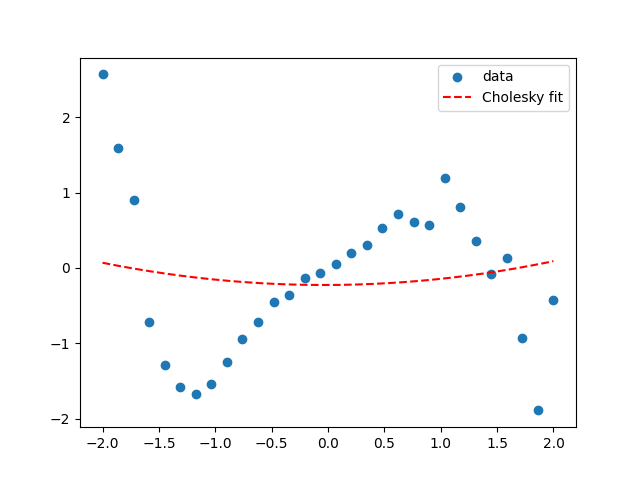
\includegraphics[width=0.75\linewidth]{../Figures/M3Chol_plot_dataset1.png}
    \end{center}

    \subsection{Cholesky plot for dataset 2 m=3}

    her er det andre plottet
    \begin{center}
    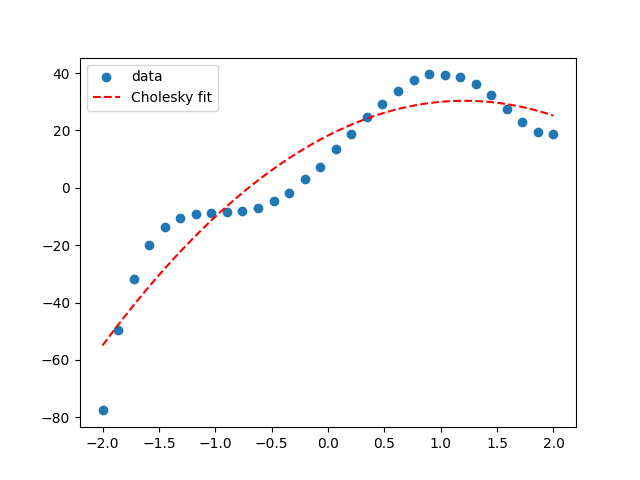
\includegraphics[width=0.75\linewidth]{../Figures/M3Chol_plot_dataset2.png}
    \end{center}


    

\end{solbox}


\section{Exercise 3}

Here I will discuss the differences







\end{document}
